\def\fasterrcnn{
    Được lấy động lực từ những điểm yếu của mô hình R-CNN \cite{girshick2014rich} và Fast R-CNN \cite{girshick2015fast}, nhóm tác giả đã nghiên cứu và phát triển mô hình Faster R-CNN \cite{ren2015faster} với trung tâm là kiến trúc mô hình Region Proposal Network (gọi tắt là RPN).
    Mô hình RPN được kỳ vọng sẽ thay thế hoàn toàn các thuật toán như Selective Search \cite{uijlings2013selective} trong kiến trúc của các mô hình two-stage giải quyết bài toán nhận diện đối tượng, hướng đến việc cải thiện không chỉ tốc độ của mô hình mà còn cải thiện về độ chính xác.

    \subsubsection*{Kiến trúc mô hình RPN}
    Mô hình RPN nhận đầu vào là ảnh với kích thước bất kỳ và trả đầu ra là toạ độ của các khu vực và xác suất khu vực đó là đối tượng nào trong các lớp đối tượng\index{lớp đối tượng}.
    Nhằm tiết kiệm chi phí tính toán, mô hình RPN dùng chung phần mô hình xương sống\index{mô hình xương sống} với Fast R-CNN.

    \begin{figure}[H]
        \centering
        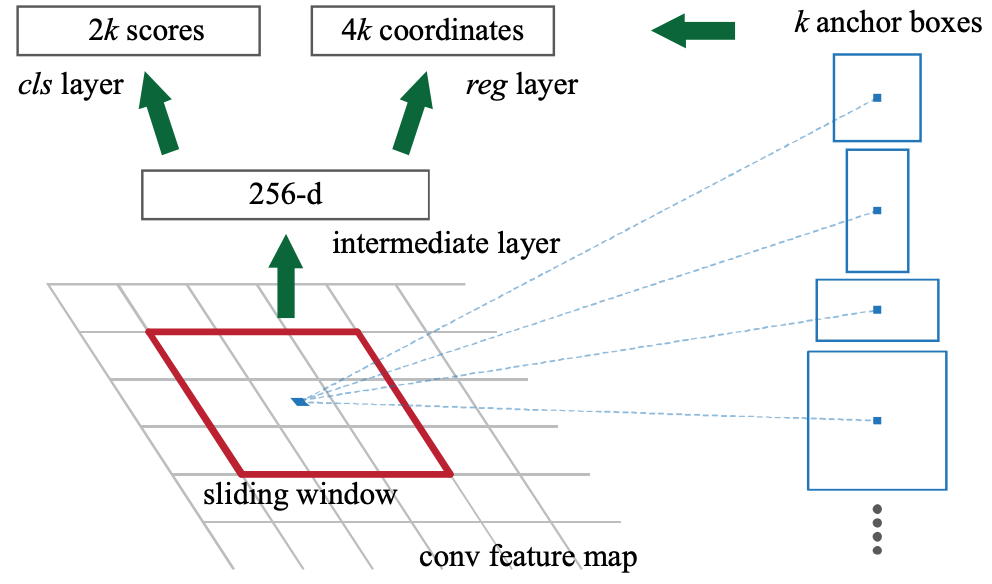
\includegraphics[width=9cm] {images/faster_rcnn_rpn}
        \caption{Kiến trúc mô hình RPN (Nguồn: \cite{ren2015faster})}
        \label{fig:faster_rcnn_rpn}
    \end{figure}
    
    \noindent
    Sau khi đưa ảnh qua mô hình xương sống\index{mô hình xương sống} và thu được một bản đồ đặc trưng\index{bản đồ đặc trưng}, mô hình RPN nhận đầu vào là bản đồ đặc trưng\index{bản đồ đặc trưng} này và trả đầu ra là các khu vực đề xuất gọi là các khu vực mỏ neo\index{khu vực mỏ neo}.
    Nhóm tác giả xây dựng phương pháp đề xuất các khu vực mỏ neo\index{khu vực mỏ neo} dựa trên kích thước và tỷ lệ giữa chiều dài và chiều rộng của khu vực mỏ neo\index{khu vực mỏ neo}.
    Cụ thể, mô hình RPN đưa bản đồ đặc trưng\index{bản đồ đặc trưng} qua một lớp Conv\index{lớp Conv} và thu được một bản đồ đặc trưng\index{bản đồ đặc trưng} mới có kích thước W x H.
    Từ đó, nhóm tác giả đề xuất ba kích thước của khu vực mỏ neo\index{khu vực mỏ neo} và ba tỷ lệ giữa chiều dài và chiều rộng của khu vực mỏ neo\index{khu vực mỏ neo} tạo ra chín khu vực mỏ neo\index{khu vực mỏ neo} với mỗi điểm ảnh\index{điểm ảnh} trên bản đồ đặc trưng\index{bản đồ đặc trưng} kích thước W x H.
    Tổng cộng trên toàn bộ bản đồ đặc trưng\index{bản đồ đặc trưng} kích thước W x H, ta thu được W x H x 9 khu vực mỏ neo\index{khu vực mỏ neo}.
    Các bản đồ đặc trưng\index{bản đồ đặc trưng} đại diện cho các khu vực mỏ neo\index{khu vực mỏ neo} này được tiếp tục đưa qua các lớp Conv\index{lớp Conv} để biến đổi về các bản đồ đặc trưng\index{bản đồ đặc trưng} mới có dạng (W x H x 9) x 1 đại diện cho xác suất khu vực mỏ neo\index{khu vực mỏ neo} đó là đối tượng và có dạng (W x H x 9) x 4 đại diện cho 4 toạ độ x của góc trái trên, y của góc trái trên, chiều dài và chiều rộng của hộp giới hạn\index{hộp giới hạn}.

    \noindent
    Một điểm mạnh của RPN so với các mô hình nhận diện đối tượng thời bấy giờ đó chính là khả năng dự đoán được các đối tượng có kích thước khác nhau và tỷ lệ giữa chiều dài và chiều rộng khác nhau nhờ vào cách cấu hình của khu vực mỏ neo\index{khu vực mỏ neo}.

    \begin{figure}[H]
        \centering
        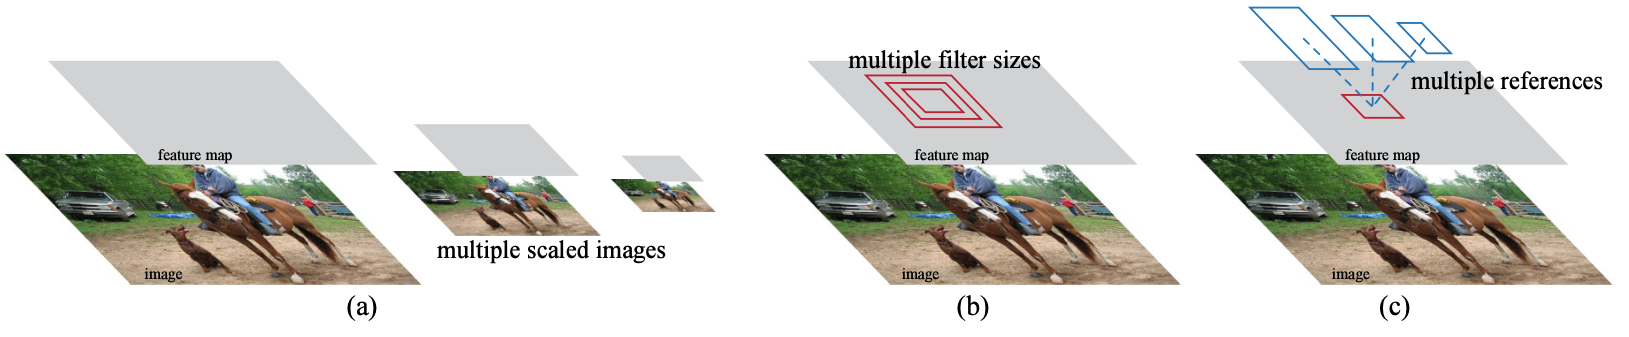
\includegraphics[width=15cm] {images/faster_rcnn_multi_scale_anchor}
        \caption{So sánh các kiến trúc xử lý vấn đề đối tượng có kích thước khác nhau và tỷ lệ giữa chiều dài và chiều rộng khác nhau (Nguồn: \cite{ren2015faster})}
        \label{fig:faster_rcnn_multi_scale_anchor}
    \end{figure}

    \noindent
    Một số kiến trúc đã được đề xuất ở thời điểm đó nhưng đều gặp phải rào cản về khối lượng tính toán lớn. \\
    - Kiến trúc đầu tiên là \textit{image / feature pyramids} sử dụng ảnh với nhiều kích thước khác nhau nhằm tạo ra bản đồ đặc trưng\index{bản đồ đặc trưng} có nhiều kích thước khác nhau.
    Kiến trúc này tốn rất nhiều chi phí tính toán do ta cần xử lý nhiều lần (thường là ba lần) với mỗi ảnh đầu vào khác nhau. \\
    - Kiến trúc thứ hai là \textit{pyramid of filters} đưa cùng một bản đồ đặc trưng\index{bản đồ đặc trưng} đầu vào qua nhiều khối Conv có kích thước của kernel khác nhau (thường là Conv với có kích thước 5x7 và Conv với có kích thước 7x5).
    Kiến trúc này tiết kiệm chi phí tính toán hơn một chút so với kiến trúc đầu tiên và thường được sử dụng kết hợp cùng với kiến trúc đầu tiên. \\
    - Kiến trúc cuối cùng là \textit{pyramid of anchors} được đề xuất trong RPN sử dụng nhiều khu vực mỏ neo\index{khu vực mỏ neo} với các kích thước khác nhau và tỷ lệ giữa chiều dài và chiều rộng khác nhau.
    Kiến trúc này chỉ tăng một lượng nhỏ chi phí tính toán nếu ta tăng số lượng khu vực mỏ neo\index{khu vực mỏ neo}, còn phần chi phí tính toán đối với bản đồ đặc trưng\index{bản đồ đặc trưng} vẫn được giữ nguyên. \\
    Phần cải tiến của RPN đối với đối tượng có kích thước khác nhau và tỷ lệ giữa chiều dài và chiều rộng khác nhau chỉ là những cải tiến tại thời điểm đó mà thôi.

    \subsubsection*{Hàm mất mát và cách huấn luyện mô hình RPN}
    Để huấn luyện được mô hình RPN, nhóm tác giả gán cho mỗi khu vực mỏ neo\index{khu vực mỏ neo} một lớp groundtruth\index{groundtruth} và thiết lập hàm mất mát\index{hàm mất mát} đối với từng khu vực mỏ neo\index{khu vực mỏ neo}.
    Nhóm tác giả gán lớp groundtruth\index{groundtruth} dương cho khu vực mỏ neo\index{khu vực mỏ neo} dựa theo hai cách sau: \\
    - Những khu vực mỏ neo\index{khu vực mỏ neo} có chỉ số IoU\index{IoU} lớn nhất đối với một groundtruth\index{groundtruth} hộp giới hạn\index{hộp giới hạn} được gán là khu vực mỏ neo\index{khu vực mỏ neo} dương. \\
    - Những khu vực mỏ neo\index{khu vực mỏ neo} có chỉ số IoU\index{IoU} lớn hơn 0.7 đối với một groundtruth\index{groundtruth} hộp giới hạn\index{hộp giới hạn} được gán là khu vực mỏ neo\index{khu vực mỏ neo} dương. \\
    Với hai cách như trên, một groundtruth\index{groundtruth} hộp giới hạn\index{hộp giới hạn} có thể gán được cho nhiều khu vực mỏ neo\index{khu vực mỏ neo} khác nhau.
    Ngoài ra, nhóm tác giả cũng gán lớp groundtruth\index{groundtruth} âm cho các khu vực mỏ neo\index{khu vực mỏ neo} không phải là dương và có chỉ số IoU\index{IoU} nhỏ hơn 0.3 đối với một groundtruth\index{groundtruth} hộp giới hạn\index{hộp giới hạn}. \\
    Từ đó, mô hình Faster R-CNN tối ưu hàm mất mát\index{hàm mất mát} sau:

    \begin{equation}
        \label{eq:faster_rcnn_loss}
        L(\{p_i\}, \{t_i\}) = \frac{1}{N_{cls}}\sum_i L_{cls}(p_i, p^{*}_i) + \lambda\frac{1}{N_{reg}}\sum_i  p^{*}_i L_{reg}(t_i, t^{*}_i).
    \end{equation}

    \noindent
    trong đó: \\
    - \textit{i} là chỉ số của từng khu vực mỏ neo\index{khu vực mỏ neo}. \\
    - \textit{$p_i$} là xác suất mà khu vực mỏ neo\index{khu vực mỏ neo} chứa đối tượng. \\
    - \textit{$p^{*}_i$} là groundtruth\index{groundtruth} của khu vực mỏ neo\index{khu vực mỏ neo} (là 1 nếu khu vực mỏ neo\index{khu vực mỏ neo} đó được gán là chứa đối tượng, là 0 nếu khu vực mỏ neo\index{khu vực mỏ neo} đó được gán là không chứa đối tượng). \\
    - \textit{$t_i$} là vector gồm 4 giá trị đại diện cho toạ độ của khu vực mà mô hình RPN đề xuất. \\
    - \textit{$t^{*}_i$} là vector gồm 4 giá trị đại diện cho toạ độ của groundtruth\index{groundtruth} hộp giới hạn\index{hộp giới hạn} tương ứng với khu vực mỏ neo\index{khu vực mỏ neo} đó. \\
    Hàm mất mát\index{hàm mất mát} trên gồm các thành phần: \\
    - \textit{$L_{cls}$}: là hàm mất mát\index{hàm mất mát} phân lớp thông thường giúp xác định khu vực mỏ neo\index{khu vực mỏ neo} có chứa đối tượng hay không. \\
    - \textit{$L_{reg}$}: là hàm mất mát\index{hàm mất mát} hồi quy đối với các khu vực mỏ neo\index{khu vực mỏ neo} dương, giúp tinh chỉnh toạ độ của khu vực mà mô hình đề xuất.
    Cụ thể, nhóm tác giả sử dụng $L_{reg}(t_i, t^{*}_i)=L_1(t_i - t^{*}_i)$ giống với hàm mất mát\index{hàm mất mát} sử dụng trong mô hình Fast R-CNN \cite{girshick2015fast}.

    \noindent
    Mô hình RPN được thiết kế để có thể huấn luyện cùng với quá trình huấn luyện nhận diện đối tượng từ đó giúp kết quả đề xuất khu vực trở nên chính xác hơn.
    Tuy nhiên, có một vấn đề nảy sinh khi sử dụng mô hình RPN cho việc đề xuất khu vực, đó là mô hình sẽ đề xuất ra nhiều các khu vực mỏ neo\index{khu vực mỏ neo} âm hơn rất nhiều so với số khu vực mỏ neo\index{khu vực mỏ neo} dương.
    Việc huấn luyện mô hình trên từng khu vực mỏ neo\index{khu vực mỏ neo} kết hợp với hiện tượng trên sẽ khiến cho tổng quan mô hình nhận diện đối tượng bị mất cân bằng dữ liệu\index{mất cân bằng dữ liệu}.
    Ngoài ra, việc huấn luyện mô hình với toàn bộ số khu vực mỏ neo\index{khu vực mỏ neo} được đề xuất ra cũng sẽ khiến cho khối lượng tính toán lớn và thời gian kéo dài quá trình huấn luyện mô hình.
    Từ đó, nhóm tác giả đề xuất việc lựa chọn ngẫu nhiên 256 khu vực mỏ neo\index{khu vực mỏ neo} trên mỗi ảnh để thực hiện việc tính giá trị hàm mất mát\index{hàm mất mát}. Việc lựa chọn này giúp tỷ lệ khu vực mỏ neo\index{khu vực mỏ neo} dương và âm trở nên cân bằng hơn và giảm thiểu bởi những phần khối lượng tính toán dư thừa.

    \subsubsection*{Sự kết hợp giữa mô hình RPN và Fast R-CNN}
    Nhóm tác giả cho rằng, việc huấn luyện mô hình RPN và Fast R-CNN cần phải diễn ra đồng thời, vì từ đó, việc chia sẻ chung thành phần mô hình xương sống\index{mô hình xương sống} Conv mới trở nên hiệu quả.

    \begin{figure}[H]
        \centering
        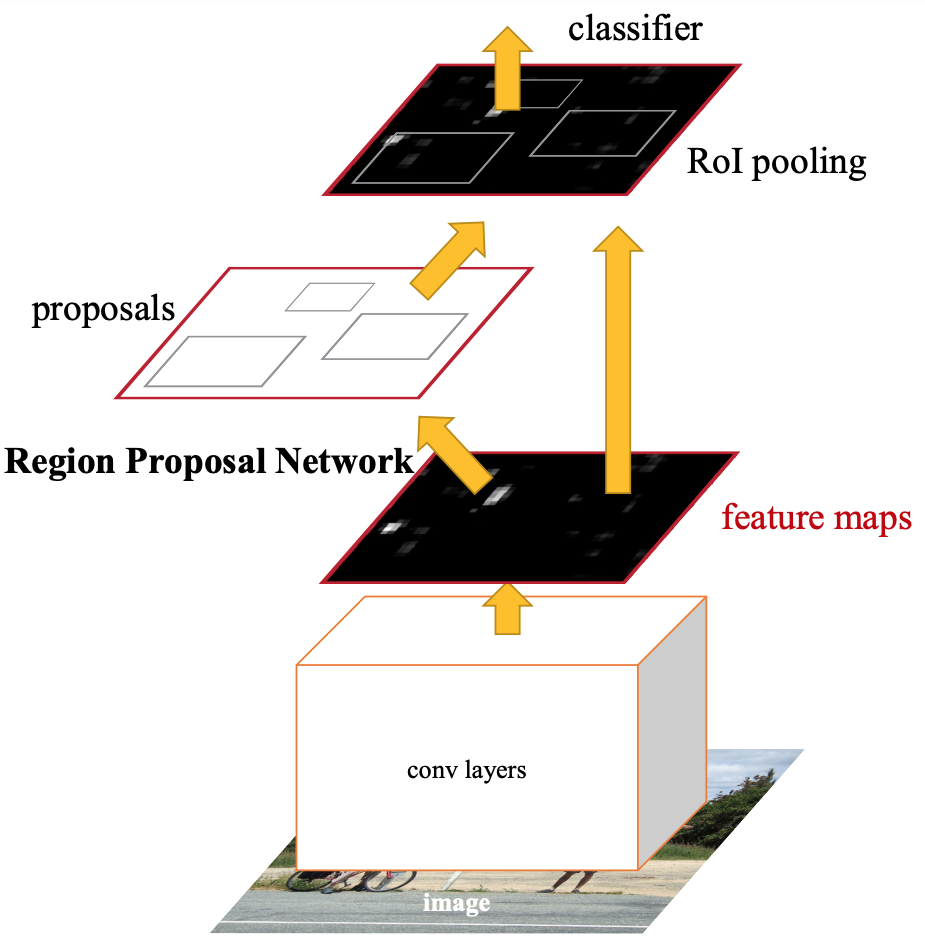
\includegraphics[width=8cm] {images/faster_rcnn_model}
        \caption{Toàn cảnh sự kết hợp của mô hình RPN và Fast R-CNN tạo ra mô hình Faster R-CNN (Nguồn: \cite{ren2015faster})}
        \label{fig:faster_model}
    \end{figure}

    \noindent
    Nhóm tác giả nêu ra ba phương án để huấn luyện mô hình RPN kết hợp với Fast R-CNN: \\
    - Cách 1: \textit{Alternating training}: Nhóm tác giả huấn luyện mô hình RPN trước sử dụng những hàm mất mát\index{hàm mất mát} của RPN nói trên.
    Sau khi huấn luyện xong mô hình RPN, tác giả sử dụng những khu vực được đề xuất bởi RPN để huấn luyện mô hình Fast R-CNN.
    Mô hình mô hình xương sống\index{mô hình xương sống} sau khi được huấn luyện bởi Fast R-CNN tiếp tục được sử dụng để huấn luyện mô hình RPN mới và vòng lặp này tiếp tục diễn ra cho đến khi kết quả của mô hình hội tụ. \\
    - Cách 2: \textit{Approximate joint training}: Phương pháp này kết hợp RPN và Fast R-CNN thành một mô hình duy nhất trong quá trình huấn luyện.
    Các khu vực được đề xuất bởi RPN được coi như là tất định đối với nhánh Fast R-CNN và khiến cho phương pháp huấn luyện này được gọi là \textit{approximate} bởi vì những thông tin từ nhánh Fast R-CNN sẽ không được cập nhật cho nhánh RPN.
    Quá trình lan truyền ngược\index{lan truyền ngược} được thực hiện độc lập giữa RPN và Fast R-CNN, riêng phần mô hình xương sống\index{mô hình xương sống} chung của RPN và Fast R-CNN được cập nhật theo giá trị hàm mất mát\index{hàm mất mát} của cả RPN và Fast R-CNN.
    Phương pháp này đạt hiệu quả thấp hơn chút so với \textit{Alternating training} tuy nhiên thời gian huấn luyện được giảm 25 - 50\%. \\
    - Cách 3: \textit{Non-approximate joint training}: Phương pháp này cải thiện được vấn đề \textit{approximate} tồn đọng của \textit{Approximate joint training}.
    Tuy nhiên, để làm được điều này, nhóm tác giả cần tinh chỉnh lại lớp RoI pooling trong Fast R-CNN để có thể update cho cả các thành phần của mô hình Fast R-CNN và RPN.
    Điều này nằm ngoài nội dung của nghiên cứu này nên nhóm tác giả không đề cập kỹ hơn.

    \noindent
    Tóm lại, nhóm tác giả dựa vào phương pháp \textit{Alternating training} và thực hiện quá trình huấn luyện gồm bốn bước như sau: \\
    - Bước 1: Nhóm tác giả khởi tạo mô hình RPN với pretrained ImageNet và huấn luyện mô hình RPN. \\
    - Bước 2: Nhóm tác giả khởi tạo mô hình Fast R-CNN với pretrained ImageNet và huấn luyện mô hình Fast R-CNN với các khu vực được đề xuất bởi RPN. \\
    - Bước 3: Nhóm tác giả khởi tạo lại mô hình RPN nhưng sử dụng phần mô hình xương sống\index{mô hình xương sống} đã được huấn luyện từ Bước 2.
    Nhóm tác giả chỉ huấn luyện những lớp riêng của mô hình RPN và không cập nhật cho phần mô hình xương sống\index{mô hình xương sống}. \\
    - Bước 4: Nhóm tác giả finetune lại những lớp riêng của mô hình Fast R-CNN với các khu vực được đề xuất bởi RPN và thu được mô hình Faster R-CNN cuối cùng. \\
    Nhóm tác giả cũng đã lặp lại bốn bước trên vài lần nhưng kết quả không thay đổi quá nhiều.

    \subsubsection*{Vấn đề tồn đọng của mô hình Faster R-CNN}
    Kết quả của mô hình Faster R-CNN và tâm điểm là kiến trúc RPN giúp thay thế thuật toán Selective Search đã giúp cho Faster R-CNN đạt độ chính xác cao hơn so với mô hình Fast R-CNN sử dụng Selective Search.
    Hơn nữa, RPN giúp cho Faster R-CNN nhanh hơn tới 10 lần so với cấu hình tương tự Fast R-CNN sử dụng Selective Search.
    Điều này giúp cho Faster R-CNN cho đến nay vẫn là một mô hình tốt để giải quyết bài toán nhận diện đối tượng, vừa đạt độ chính xác cao, vừa có tốc độ tương đối tốt.
    Tuy nhiên, cho đến thời điểm thực hiện luận văn này, đã có nhiều mô hình khác hiện đại hơn chỉ ra những vấn đề tồn đọng của Faster R-CNN như độ chính xác cần phải cải thiện thêm hay tốc độ chưa đạt đến ngưỡng chạy trong thời gian thực. 
}